\subsection{Análisis Espectral y Ancho de Banda (Modulación Q-PSK)}
Para determinar el ancho de banda del sistema en Envolvente Compleja (EC), se analizó la Densidad Espectral de Potencia (PSD) de la señal modulada Q-PSK. Como se observa en la Figura \ref{fig:psd_qpsk}, el lóbulo principal del espectro está delimitado por "valles" o cruces por cero (nulos) claramente definidos en la escala logarítmica.

\begin{figure}[H]
    \centering
    \subfloat[Cruce por cero en el extremo negativo.]{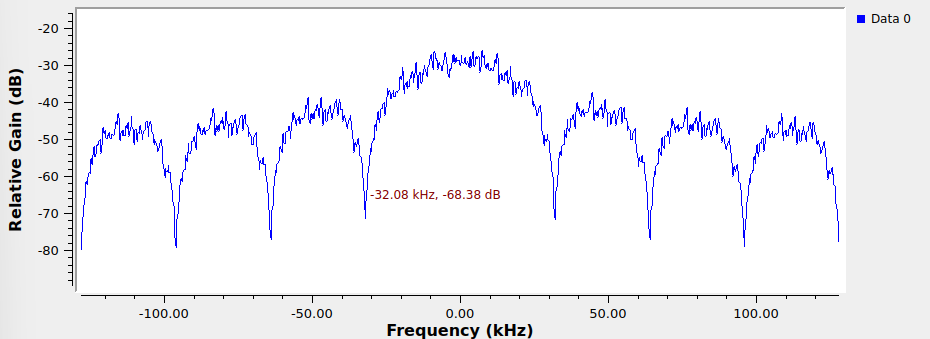
\includegraphics[width=0.48\linewidth]{imagenes/ancho_de_banda_extremo_negativo.png}\label{fig:psd_neg}}
    \hfill
    \subfloat[Cruce por cero en el extremo positivo.]{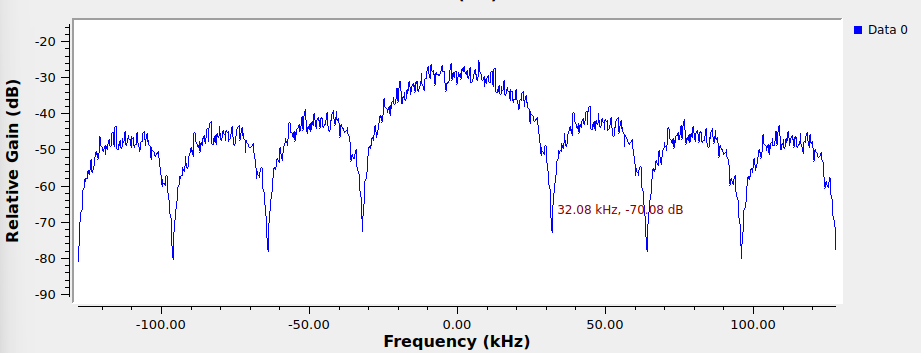
\includegraphics[width=0.48\linewidth]{imagenes/ancho_de_banda_extremo_positivo.png}\label{fig:psd_pos}}
    \caption{Ubicación de los nulos espectrales en la Densidad Espectral de Potencia (PSD) para Q-PSK.}
    \label{fig:psd_qpsk}
\end{figure}

Las mediciones experimentales mediante los cursores de GNU Radio indican que el primer nulo espectral a la izquierda ocurre en $-32.08$ kHz y el primer nulo a la derecha en $+32.08$ kHz. Matemáticamente, en modulaciones digitales con conformación de pulso rectangular, la envolvente del espectro obedece a una función del tipo $\text{sinc}^2(f/R_s)$. Por lo tanto, los cruces por cero teóricos en escala lineal se ubican de manera exacta en los múltiplos enteros de la tasa de símbolos ($R_s$).

Dado que el flujograma se configuró con una tasa de símbolos $R_s = 32$ kBd, la caída de potencia en $\pm 32$ kHz valida el modelo teórico. En consecuencia, se concluye que el ancho de banda en banda base (distancia desde $0$ Hz hasta el primer cruce por cero) es directamente igual a la tasa de símbolos del sistema: $BW_{EC} = 32$ kHz.

\subsection{Validación del Mapeo Vectorial y Efectos del Canal}
Una vez establecido el diseño del transmisor, se procedió a verificar la correcta ubicación espacial de los símbolos generados a partir de la fuente de datos. La Figura \ref{fig:evidencia_qpsk} contrasta la configuración del bloque \textit{Vector Source} con la salida real obtenida en el sumidero de constelación.

\begin{figure}[H]
    \centering
    \subfloat[Configuración del vector en GNU Radio.]{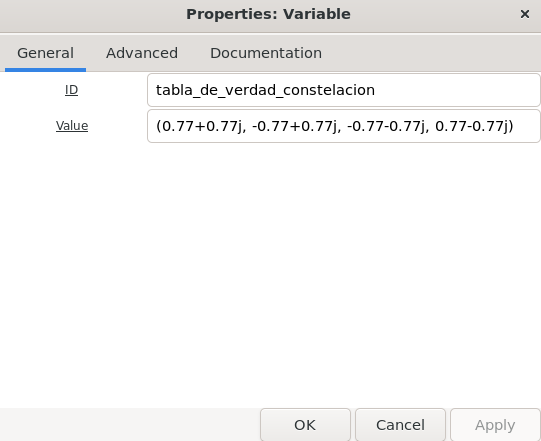
\includegraphics[width=0.55\linewidth]{imagenes/tabla_de_verdad.png}\label{fig:vector_config}}
    \hfill
    \subfloat[Constelación Q-PSK bajo efecto del canal AWGN.]{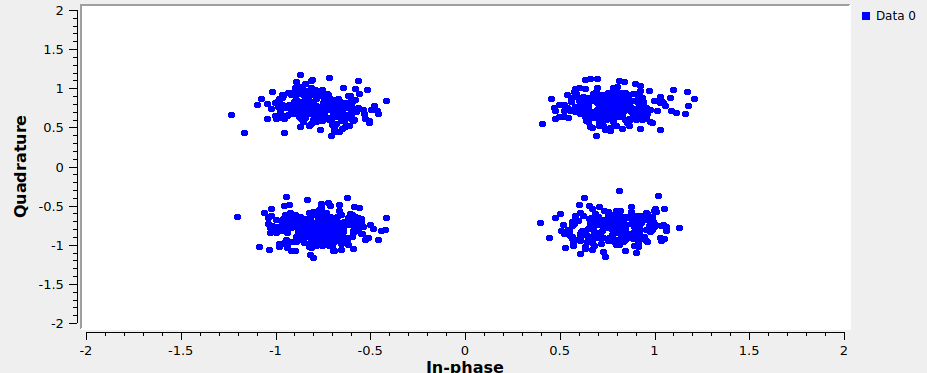
\includegraphics[width=0.40\linewidth]{imagenes/constelaciones.png}\label{fig:const_grafica}}
    \caption{Evidencia de la configuración vectorial y verificación en el plano complejo.}
    \label{fig:evidencia_qpsk}
\end{figure}

Como se evidencia en la Figura \ref{fig:const_grafica}, la salida del sistema coincide perfectamente con las cuatro coordenadas teóricas programadas ($\pm 0.77 \pm 0.77j$). Adicionalmente, la dispersión observada (formación de "nubes" alrededor de los puntos ideales) confirma la correcta emulación del canal mediante la adición de Ruido Gaussiano Blanco Aditivo (AWGN). Esta dispersión permite validar de forma cualitativa la robustez de la modulación Q-PSK: al mantener una distancia euclidiana amplia entre los 4 símbolos, el sistema es menos propenso a errores de decisión en el receptor.

\subsection{Análisis Comparativo: Q-PSK vs. M-PSK}
% [NOTA PARA JUAN: Este párrafo está listo para que lo completes en cuanto Valentina y Jordy suban sus resultados del M-PSK base].
Al contrastar el esquema Q-PSK ($M=4$) con la implementación del esquema M-PSK base, se evidencian los compromisos de diseño en las comunicaciones digitales. Mientras que el Q-PSK transmite $2$ bits por símbolo ($R_b = 64$ kbps para $R_s = 32$ kBd), el esquema M-PSK de orden superior... (completar con la comparativa de velocidades y el impacto en la distancia euclidiana frente al ruido).